%------------------------------------------%
% Cannabis Data Science
% Date: 12/15/2021
%------------------------------------------%
\documentclass[xcolor={dvipsnames}]{beamer}
\hypersetup{pdfpagemode=FullScreen}
\mode<presentation>{
  \usetheme{Boadilla}
  \usecolortheme{orchid}
  \usefonttheme{default}
  \setbeamertemplate{navigation symbols}{}
  \setbeamertemplate{caption}[numbered]
} 
\usepackage[english]{babel}
\usepackage[utf8x]{inputenc}
\setbeamersize{text margin left=0.5in,text margin right=0.5in}

\usepackage[dvipsnames]{xcolor}
\definecolor{DarkGreen}{RGB}{2, 48, 32}
\definecolor{CalyxGreen}{RGB}{34, 153, 84}
\definecolor{DarkOrange}{RGB}{199, 0, 57}
\definecolor{LightOrange}{RGB}{255, 87, 51}
\definecolor{LightGreen}{RGB}{218, 247, 166}
\definecolor{LightYellow}{RGB}{255, 195, 0}

\setbeamercolor*{palette primary}{bg=LightGreen, fg = DarkGreen}
\setbeamercolor*{palette secondary}{bg=LightGreen, fg=DarkGreen}
\setbeamercolor*{palette tertiary}{bg=LightGreen, fg = DarkGreen}
%\setbeamercolor*{palette quaternary}{bg=myNewColorD, fg = green}

%------------------------------------------%
% Packages
%------------------------------------------%
\usepackage{amsmath}
\renewcommand*\footnoterule{} %No sperating line on footnote
\usepackage{mathtools} %ANNOTATING EQUATIONS
\usepackage{hhline} %DOUBLBARS
\usepackage[super]{nth}
\usepackage{graphicx, caption, subcaption}

%------------------------------------------%
% Commands
%------------------------------------------%
\newcommand\T{\rule{0pt}{2.5ex}} %TOPSTRUT
\newcommand\B{\rule[-1.25ex]{0pt}{0pt}} %BOTTOMSTRUT
\newenvironment<>{varblock}[2][.9\textwidth] %RESIZED BLOCKS
  {\setlength{\textwidth}{#1}
  \begin{actionenv}#3
    \def\insertblocktitle{#2}\par
    \usebeamertemplate{block begin}}
  {\par\usebeamertemplate{block end}
  \end{actionenv}}
\defbeamertemplate{enumerate item}{largeball} %LARGE BALLS
{\begin{pgfpicture}{-1ex}{-0.65ex}{1.5ex}{1.5ex}
\usebeamercolor[fg]{item projected}
{\pgftransformscale{2.5}\pgftext{\Large\pgfuseshading{bigsphere}}}
{\pgftransformshift{\pgfpoint{0pt}{0.5pt}}
\pgftext{\usebeamerfont*{item projected}\small\insertenumlabel}}
\end{pgfpicture}}
\usepackage{tikz} % FANCY ARROWS
\usepackage{xparse}
\NewDocumentCommand\UpArrow{O{2.0ex} O{black}}{%
   \mathrel{\tikz[baseline] \draw [->, line width=0.5pt, #2] (0,0) -- ++(0,#1);}} % FANCY UPARROW
\NewDocumentCommand\DownArrow{O{2.0ex} O{black}}{%
   \mathrel{\tikz[baseline] \draw [<-, line width=0.5pt, #2] (0,0) -- ++(0,#1);}} % FANCY DOWNARROW
%\vskip 1cm
\makeatletter
\newcommand{\LeftEqNo}{\let\veqno\@@leqno}%LEFT EQUATION #'s
\makeatother

\renewcommand{\arraystretch}{1.7}

%------------------------------------------%
% Title
%------------------------------------------%
\title[\textbf{Meetup}]{}
\author{Cannabis Data Science}
\institute[]{\Large \textbf{Meetup}}
\date{December \nth{15}, 2021}
\begin{document}
\begin{frame}{}
  
\includegraphics[scale=0.075]{images/logos/cannlytics_logo_with_text_light.png}
  \titlepage
\end{frame}

%------------------------------------------%
% Research Question
%------------------------------------------%
\section{Research Question}

\begin{frame}{}

{\large \textbf{Research Question}: What is the \textit{underlying} relationship between dispensaries per capita and revenue per dispensary?}\vspace{0.5\baselineskip}\\

\begin{figure}
    \begin{subfigure}[t]{.8\textwidth}
      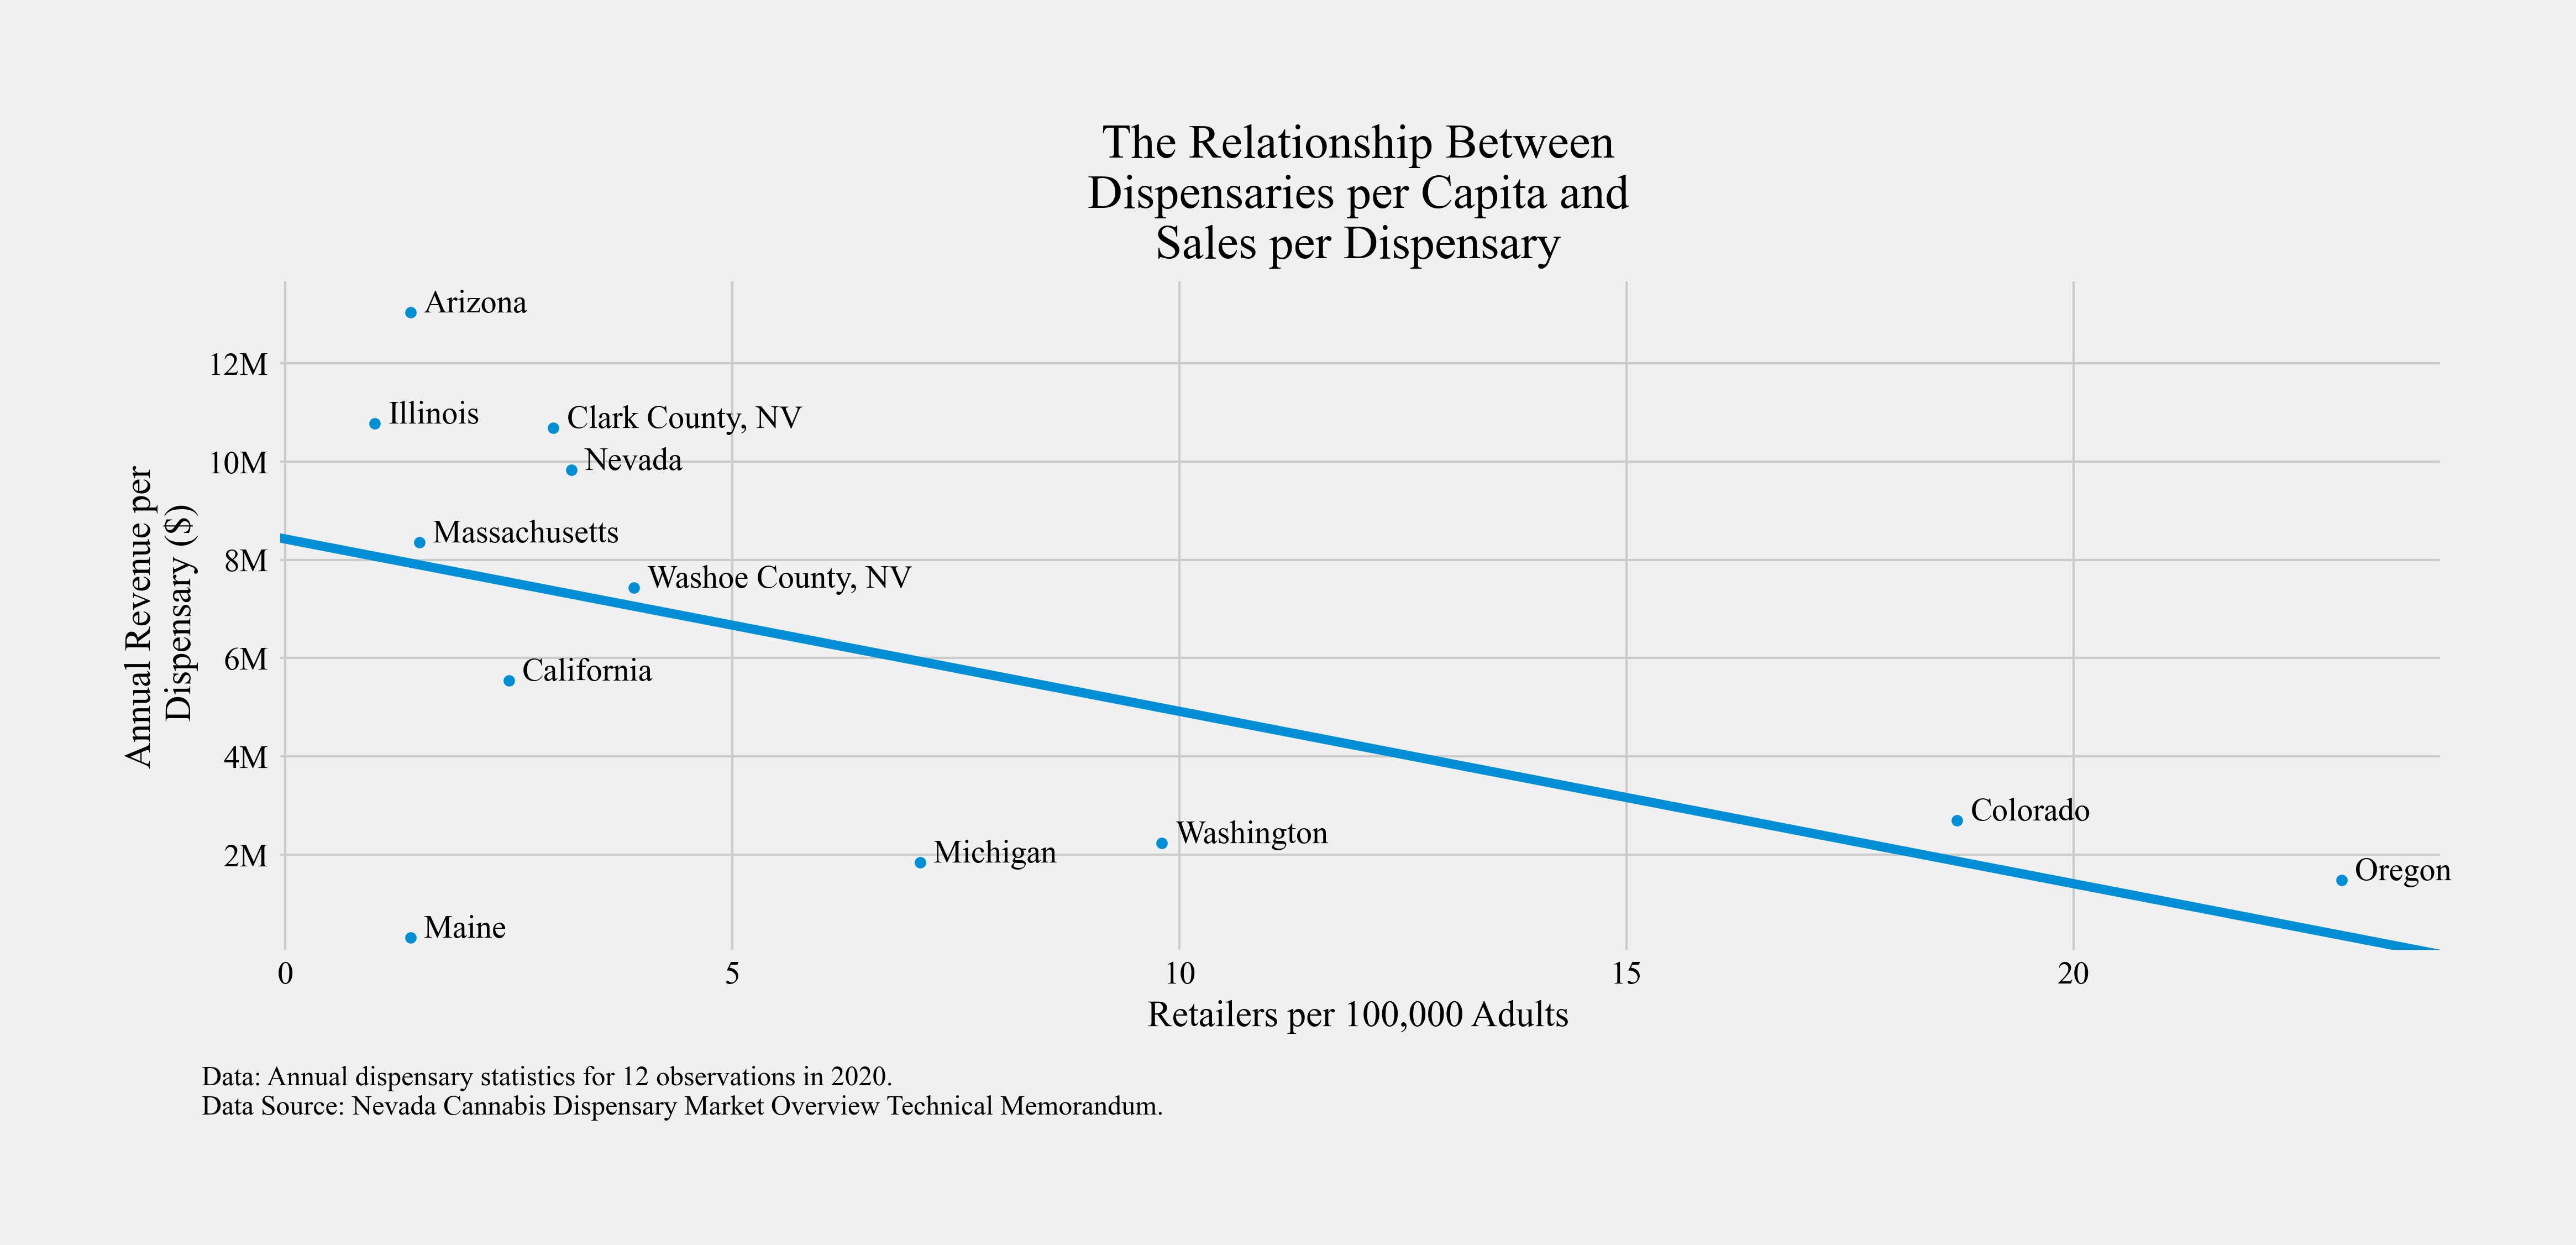
\includegraphics[width=\textwidth]{images/revenue_per_retailer_to_retailers_per_100_000.png}
    \end{subfigure}
    
    \begin{subfigure}[t]{.5\textwidth}
      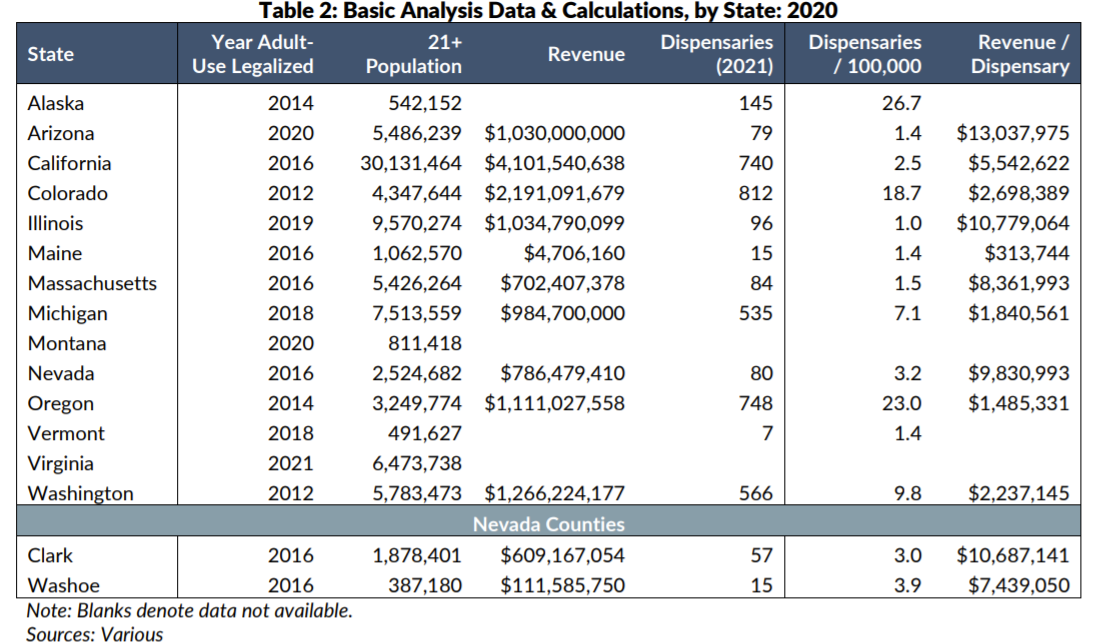
\includegraphics[width=\textwidth]{images/dispensary_statistics.png}
      \caption*{\tiny Source: Nevada Cannabis Dispensary Market Overview Technical Memorandum}
    \end{subfigure}
\end{figure}


\end{frame}

%------------------------------------------%
% Theory
%------------------------------------------%
\section{Economics}

\begin{frame}{}

\begin{figure}
    \begin{subfigure}[t]{.3\textwidth}
      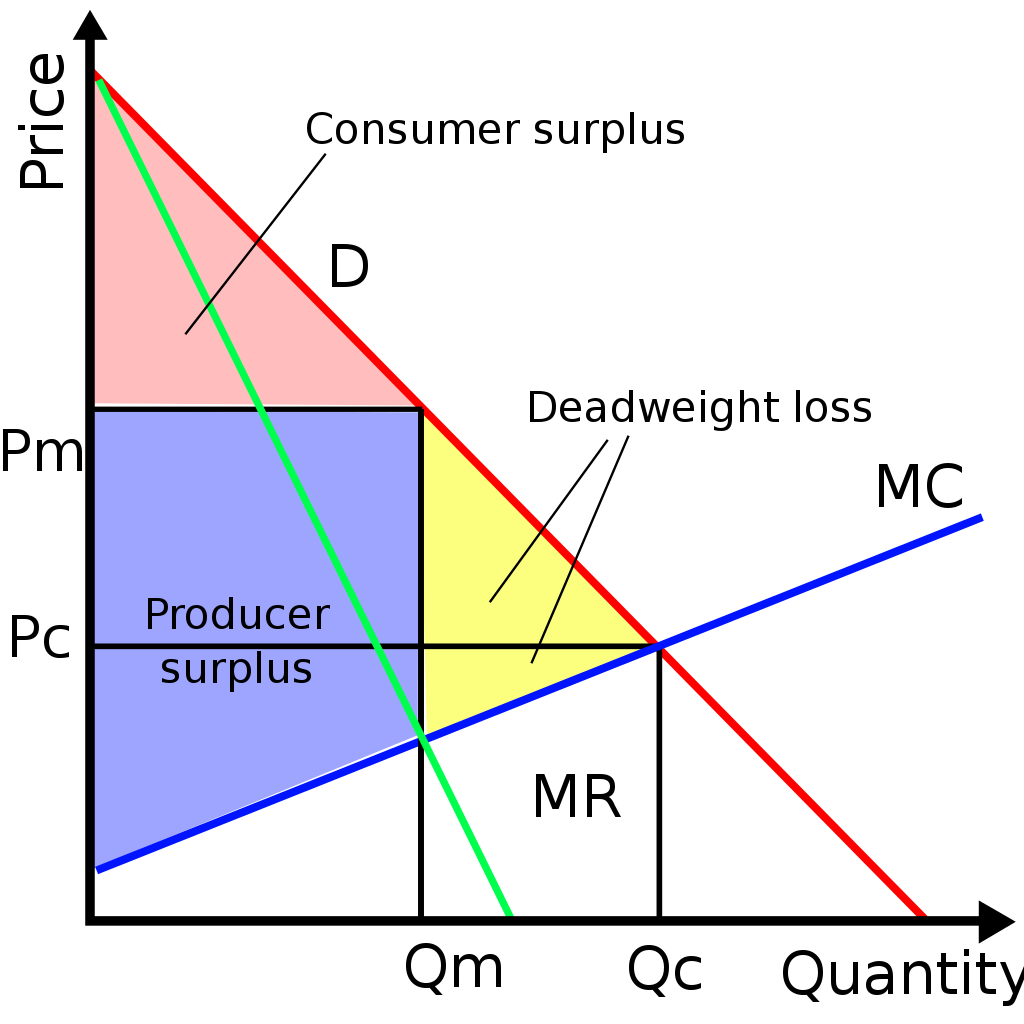
\includegraphics[width=\textwidth]{images/monopoly-surpluses.png}
      \caption*{\scriptsize A market with a monopoly\newline\tiny SilverStar at en.wikipedia}
    \end{subfigure}
\end{figure}

{\large \textbf{Industrial Organization}}

\vspace{.75\baselineskip}

\begin{itemize}

\item Seminal work by Edward S. Mason, Joe Bain, and George Stigler.

\vspace{.75\baselineskip}

\item Topics: Collusion, regulatory capture, antitrust policy, etc.

\vspace{.75\baselineskip}

\item Structure, Conduct, and Performance paradigm.

\end{itemize}


\end{frame}

%------------------------------------------%
% Market Structure
%------------------------------------------%
\begin{frame}{}

{\large \textbf{Market Structure}}

\vspace{.75\baselineskip}

{\scriptsize
\begin{tabular}{ |l|l|l|l|l|  }
 \hline
 Market Structure	& Firms & Barriers & Market Power & HHI \\
 \hline
Perfect Competition & $\infty$ & None & None & 0\\
\hline
Monopolistic Competition & Many  & Low & Low & Below 2,500\\
\hline
Oligopoly & Few & High & Medium & Above 2,500\\
\hline
Monopoly & 1 & Blocked & High & 10,000 \\
 \hline
\end{tabular}
}

\vspace{.75\baselineskip}

{\footnotesize ``\textit{Transactions that increase the HHI by more than 200 points in highly concentrated markets are presumed likely to enhance market power under the Horizontal Merger Guidelines issued by the Department of Justice and the Federal Trade Commission.}''}

{\tiny Source: https://www.justice.gov/atr/herfindahl-hirschman-index }

\end{frame}

%------------------------------------------%
% Measures
%------------------------------------------%

\begin{frame}{}

{\large \textbf{Structure, Conduct, and Performance}}

\vspace{.75\baselineskip}

\begin{itemize}

\item Measures:

\vspace{.75\baselineskip}

\begin{itemize}
\item \textbf{N-firm concentration ratio}, the combined market share of the N largest firms in the market.

$$CR_N = \sum_{n=1}^{N} s_n$$

where $s_n$ is the market share of the $n$th largest firm.

\vspace{.75\baselineskip}

\item \textbf{Herfindahl-Hirschman index}, a commonly accepted measure of market concentration:

$$HHI = s_1^2 + s_2^2 + \ldots\ + s_n^2$$

where

\vspace{.75\baselineskip}

\begin{itemize}

\item $n$ is the number of firms in the market,

\vspace{.75\baselineskip}

\item $s_n$ denotes the market share of the $n$th firm.

\end{itemize}

\end{itemize}


\end{itemize}

\end{frame}

%------------------------------------------%
% Panel Data
%------------------------------------------%
\section{Panel Data}

\begin{frame}{}

{\large \textbf{Panel Data}}\vspace{0.5\baselineskip}\\

A panel has the form

\begin{figure}
    \begin{subfigure}[t]{.5\textwidth}
      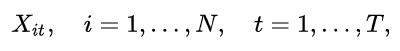
\includegraphics[width=\textwidth]{images/panel.png}
    \end{subfigure}
\end{figure}

where $i$ is the individual dimension and $t$ is the time dimension.\vspace{0.5\baselineskip}\\

A general panel data regression model is written as

\begin{figure}
    \begin{subfigure}[t]{.3\textwidth}
      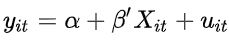
\includegraphics[width=\textwidth]{images/regression.png}
    \end{subfigure}
\end{figure}

where

\begin{figure}
    \begin{subfigure}[t]{.25\textwidth}
      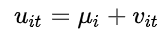
\includegraphics[width=\textwidth]{images/errors.png}
    \end{subfigure}
\end{figure}

Estimation with a \textbf{fixed effects} or \textbf{random effects} model depends on assumptions about $\mu_i$, the individual-specific, time-invariant effects.

\end{frame}


%------------------------------------------%
% Takeaway
%------------------------------------------%

\section{Conclusion}

\begin{frame}{}

\begin{center}
\begin{minipage}{3.85in}

\includegraphics[width=.25in]{images/prayer.png} Thank you for coming.\vspace{0.5\baselineskip}\\


Take some time and discuss any conclusions drawn.
\end{minipage}
\end{center}

\end{frame}

%------------------------------------------%
\end{document}
%------------------------------------------%
